\section{Application: ISP Behavior}



\subsection{Web Tripnets: Detecting ISP Content Injection}

\meddle can be configured to detect in-flight Web-page changes. 
This problem of HTTP interference was first highlighted by Reis~\etal~\cite{reis:tripwires}. 
The authors demonstrated that although a small percent of users were affected by in-flight changes, those changes tend to introduce vulnerabilities including cross-site scripting (XSS) attacks~\cite{reis:tripwires}. 
They proposed and deployed \emph{Web Tripwires}, a Javascript code to detect in-flight page changes. 
The main limitation of \emph{Web Tripwires} is that it requires each Web site to modify their content to include a tripwire.

In \meddle, we extended tripwires to alleviate this limitation. 
Namely, we use the HTTP proxy present in \meddle to inject a tripwire on \emph{any} page without requiring support from Web site developers -- an approach we call a \emph{Web Tripnet}.

\tbd{Do we still want to go ahead with the transparent proxy approach mentioned in \ref{fig:tripnets}}

\begin{figure}
\centering
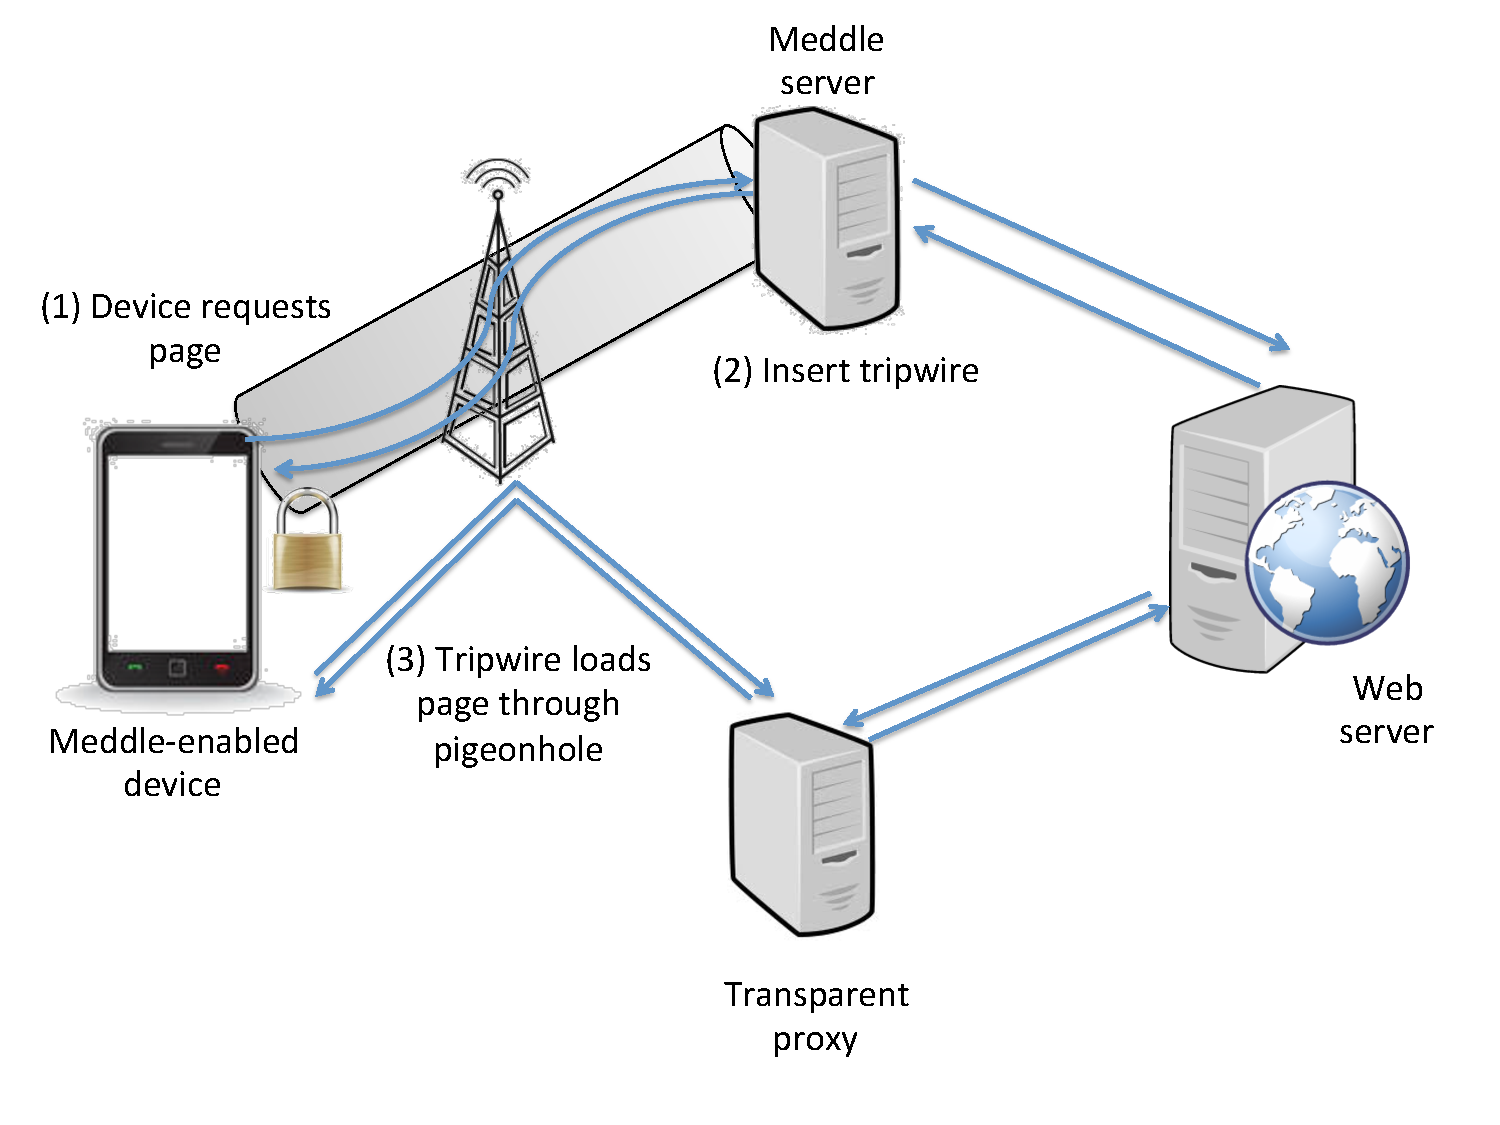
\includegraphics[width=0.9\linewidth]{figures/tripnet.pdf}
\caption{Overview of the \meddle Web-tripnet. A Web page is loaded
through the VPN tunnel, where a meddlebox inserts a Web tripwire. The
tripwire causes the browser to reload the Web page using the address of a
transparent proxy server that is accessed using an unencrypted connection.
After the proxied version of the page is loaded, the browser or a meddlebox
can compare the two pages to identify potential interference. }
\label{fig:tripnet}
\end{figure}

\noindent\textbf{Sites tested.}

\noindent\textbf{Page modification/injection.} Cases of manipulation of text content.

\noindent\textbf{Content modification.} Downsampling, e.g.

\noindent\textbf{Implications.} 


\subsection{App-Agnostic Replay: Detecting Service Differentiation}

Overview of the approach and challenges. \meddle allows us to capture 
traces from mobile devices over both \wifi and cell, meaning we can model 
behavior from either medium. \meddle also serves as a convenient location 
to conduct replay experiments. The challenge is how to capture and replay 
the salient features of application traffic such that it will be subject to differentiation 
from middleboxes. State what we can reproduce (timings, sequence of bytes, ports and source IPs) 
and what we cannot (destination IPs from client). Challenges with UDP. Challenges 
with different network conditions. Differences from Glasnost.

\textbf{Graph}: If we find a case of difference between \wifi and cell, plot it here.

Assumptions: ISPs will differentiate traffic based on hostname, IP addresses, ports, total number of 
connections, payload signatures, total bandwidth, time of day, ... \tbd{anything else?}

\noindent\textbf{Approach and feasibility.}
Description of adopted replay approach and tests to show validity.

\textbf{Graph}: Similarity score for network traffic in setting where we know there is no differentiation. 
Score can include overall throughput, latency characteristics, loss, packet timings.

\noindent\textbf{Wide-area testing.} Networks tested, observed behavior.

\textbf{Table}: each row is an app, each column is an ISP, each cell is a marker indicating what kind of 
differentiation is happening

\textbf{Graph}: Plot showing a sequence of traces that demonstrates what this differentiation looks like



\noindent\textbf{Content modification.} Downsampling, e.g.

\noindent\textbf{Implications.} 